%% 2015/11/30
%% by Kendall Pitts, Curtis Sunley, Sophia Thach, Lauren Whiteshell
%% CSC 490 - Senior Project

%%*************************************************************************

\documentclass[twocolumn,12pt]{article}
\usepackage[toc,page]{appendix}
\usepackage[english]{babel}
\usepackage{blindtext}
\usepackage{booktabs}
\usepackage[font=small,labelfont=bf]{caption}
\usepackage{color}
\usepackage[margin=1in]{geometry}
\usepackage{listings}
\usepackage{pdfpages}
\usepackage{verbatim}

\begin{document}

\title{\bf Team Firefoot: Project MedaWiGi}

\author
	{
	Kendall Pitts\\
	klpitts@uncg.edu\\
	\and
	\vspace{3pt}
	\bf Fall 2015\\
	\bf Instructor: Jing Deng\\
	\bf j\_deng@uncg.edu\\
	\and 
	Curtis Sunley\\
	casunley@uncg.edu
	\and 
	Sophia Thach\\
	s\_thach@uncg.edu
	\and 
	Lauren Whiteshell\\
	lkwhites@uncg.edu
	}
	
\date{}
\maketitle

\begin{abstract}
With this project, our overall goal was to create a web application that users could utilize in helping track important medical information. This would allow a wide variety of data about the user to be recorded. Some examples include medical insurance, doctor's appointments, past and current medications, medical conditions, and more. Not only did we want future users to have the capability of tracking their own health status, we wanted to allow them to keep records of other people's medical information. This would include the power to create profiles for dependents without the hassle of registering them to the website. In addition, we wanted users to have the ability to link to other users, allowing them to share their medical data. In the end, we accomplished many of our goals, but not without limiting the scope of the project.

\end{abstract}

\section{Introduction}
The product as a whole gives the users the ability to document various medical information through several means. A journal was implemented to allow the users to keep record of any number of things, having the flexibility for them to specify their own topic. The journal could be used as a food diary, a means to track any medical condition one has, a way to record allergic reactions, an appointment reminder, and more. With this journal, date and time should be specified upon entry. Therefore, the journal entries could then be used to populate the embedded calendar. This calendar gives the users a convenient means of viewing their created events, not only for themselves but for any profile they may be keeping track of as well. From the calendar, users can view all past, present, and future events on the specified dates. In addition, they may click on a particular event to view any information associated with that event. 

To account for the remaining information, tables were utilized for easy record-keeping and beneficial aesthetic properties. The application allows medications, immunizations, allergies, medical conditions, medical insurance, and contacts to be documented. In addition to tracking one’s own medical information, the application gives users the capability to create profiles for non-registered users, as well as link to registered users. One can connect with a profile associated with a registered user by adding that particular user by email. This may be desirable if one’s spouse owns their own account and they need to have access to each other’s medical data. On the other hand, if a user has a dependent (i.e. child) that they do not wish to register as a user but still need to record their medical status, they can then create the profile without the hassle of creating an entire account for that dependent. It is worth noting that the maximum number of additional people one individual can connect with is ten.  

\section{Background}
Though research showed there are several applications designed to help document and keep track of appointments, medical records, and other medical data, there are few applications that combine every functionality into one place without accessibility limitations. Many applications focus on keeping track of medical records directly through the patient's health care providers. Our goal was to create a patient-centered web application with easy accessibility from any internet-enabled device. We wanted a simplistic way for patients to document all necessary medical data without the confusion of using multiple applications and without the restriction of relying on health care providers. 

One big decision we made as a team was deciding to write the program for the web instead of as a desktop application. We, as a group, were not experienced in web development, and this served as a valuable learning opportunity. In addition, we wanted to avoid the device limitation that other applications faced. While some of the applications researched were only accessible via an Android mobile device or Apple device, our decision to create a web application allowed the end product to be accessible from any number of devices, as long as it could access the internet.

To accomplish this project, we initially made the decision to use Java as our programming language. The goal was to use a language we were all familiar with to ensure that we could spend more time on learning the version control software, GitHub, as well as creating the product with as great of functionality as possible. But after further research, it was decided to use PHP instead, given that PHP would be more efficient than Java for our project. It was also an additional learning experience for the group since no one had previously worked with PHP. It being a server-side scripting language designed specifically for web development, we used PHP as the script that interacted with the database, inputting and retrieving the data that was stored. In addition, we utilized HTML, CSS, and JavaScript to handle the client side. Javascript was used as our client-side script, used to validate and encrypt the data entered before it is stored in the database. HTML and CSS were used to display decrypted data from the database in an aesthetically pleasing and user-friendly way. This allowed the user to have a better user experience with the data that they inputted in the system.

To assist in handling the high volume of user profiles with our project, we had originally decided to utilize Drupal, a content management framework (CMF) and a content management platform (CMP) that has powerful developer-friendly tools that are used to develop complex sites. In addition, we had picked LDAP (Lightweight Directory Access Protocol), an open, vendor-neutral, industry standard application protocol for accessing and maintaining distributed directory information services over an Internet Protocol (IP) network, to help in managing the portal access of registered users (e.g. one's spouse) and non-registered users (e.g. dependents or children). Unfortunately, given the timeframe of the project, it was determined there was not enough time to add an excess of new technologies to learn. This compromise allowed us to advance further in our actual project construction.

\section{System Model}
Most web developers and frameworks follow this Model-View-Controller (MVC) model when creating a web-page to create code consistency and assist with security of the website.  This system prevents one file with a hodge-podged source code and it creates easier readability because it is a panoply of smaller files. 

Models are basically how objects or tables are defined within databases.  Models are defined by its characteristics or columns.

Views are the pages that the user sees and interacts with.  Typically, they contain HTML, CSS, and JavaScript.  These pages also shows how the models are displayed to the user and is where the system gets user input (with HTML forms).

Controllers are the most powerful of the structures because it is the centralized hub that communicates between the Models, Views and the Server.  Controllers like in our project contain server-side language.

\begin{figure}[!htb] 
	\centering
	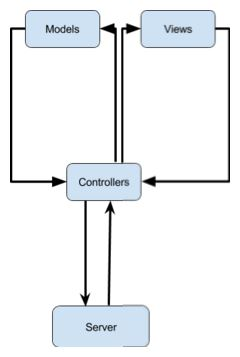
\includegraphics[scale=1]{./490/MVC3.jpg}
	\caption{General MVC structure for web development.}
\end{figure} 

\section{Literary Review}
In preparation for our own design we investigated similar applications already on the market and chose three of the most popular, as well as an additional application with which members of our group have had personal experience. The most popular applications attempted to be comprehensive in their record-keeping. They include iBlueButton, Track My Medical Records, and My Medical. The other application, Migraine Buddy, is targeted toward a specific condition. These four instances include a mixture of free and priced applications, as well as applications that may include additional charges. Further descriptions of each application are given below, comparing them to our product.

\subsection{iBlueButton}
The first application we looked at, iBlueButton, was a provider and institutional specific application created by a federal initiative to provide comprehensive access to healthcare records via mobile devices (Android and iOS). Some of its features include the ability to attach notes to static displays and a dictionary of medical terms. From our list of researched case studies, iBlueButton is the only application that pools medical documents generated by multiple entities. The other applications require users to input their own data. Therefore, iBlueButton would have a greater concern for security than the other applications, given that it interfaces with multiple entities. Though the initial download is free, additional charges do apply. There is also an option for unlimited use: consumers can access this at \$9.99 while providers must pay \$49.99 for unlimited access.  Given the device limitations, additional charges, and its need for security for interfacing between multiple entities, iBlueButton least resembles our design \cite{ibluebutton}.

\begin{figure}[!htb] 
	\centering
	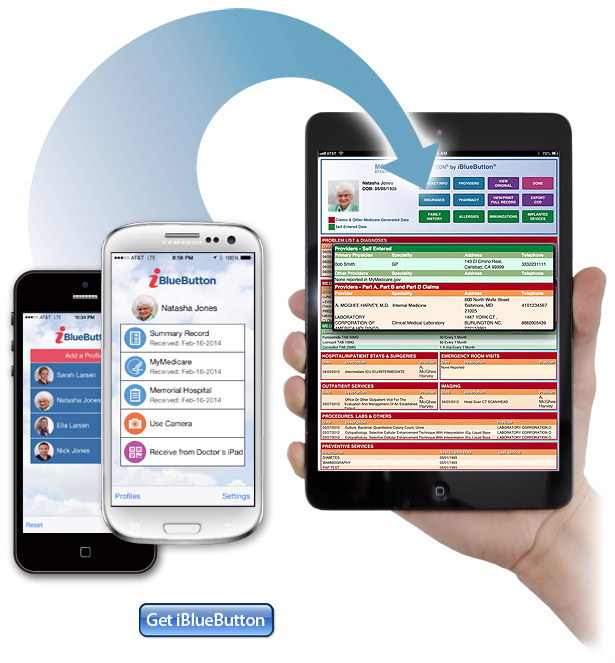
\includegraphics[scale=.2]{./490/consumer.jpg}
	\caption{iBlueButton provides comprehensive access to healthcare records.}
\end{figure}

\subsection{My Medical}
My Medical is the most expensive option on our list with a price of \$19.99, however it combines the professional accounting of iBlueButton with sleek functionality. It provides the same convenience for informal medical information that iBlueButton provides for more official documents. Although it requires the user to input a certain amount of their own data, it also supports industry standards so that all records are compatible between systems. In addition, it exists independently of any medical organizations. Additional functionalities include having the option to upload documents (i.e. x-rays), integrating the user's device's calendar, performing data analysis, and containing a dictionary of medical terms. Unfortunately, My Medical is limited to Apple devices \cite{mymedical}.

\begin{figure}[!htb] 
	\centering
	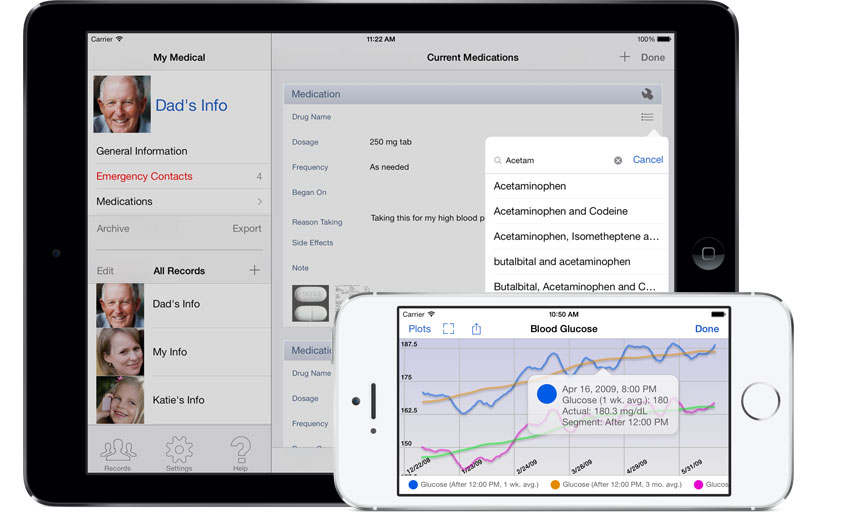
\includegraphics[scale=.2]{./490/splash_ios.jpg}
	\caption{My Medical performs data analysis.}
\end{figure}

\subsection{Track My Medical Records}
Track My Medical Records is similar to iBlueButton in that it was created to provide comprehensive access to healthcare records via mobile devices. It's primary difference lies in how the data is populated in the application. Medical records are not obtained from healthcare providers. Instead, the user must enter the data themselves. This application lacks the doctor/patient interface of the other application, giving security a lower priority. In addition, the application is free, it does not face the device limitations that the previously mentioned applications did, and because data entry is the responsibility of the user, it avoids the medical jargon that appears in more official documents. Given that the user can access the application from any device, the application does not store the data on the user's device,  and the user populates the medical data themself, Track My Medical Record most closely resembles our design. However, it does provide some data analysis, similar to My Medical, that our application does not provide \cite{freehealthtrack}.

\begin{figure}[!htb] 
	\centering
	
\includegraphics[scale=.4]{./490/card-with-words.png}
	\caption{Track My Medical Records can be accessed from any device.}
\end{figure}

\subsection{Migraine Buddy}
Migraine Buddy is a condition-specific application designed to allow users to track migraines. Much like a migraine journal, it helps users record their migraines, date when they occur and how long they last, list accompanying symptoms, specify pain intensity and location, and more. With the given information, the application provides a summary report showing top migraine triggers, average duration of migraines, a detailed summary of when migraines most commonly occur, and other helpful data. Our product lacks these analysis capabilities, but it provides greater span of functionality not being limited to a particular condition. Our application allows users to keep track of a wide range of medical data \cite{migrainebuddy}.

\begin{figure}[!htb] 
	\centering
	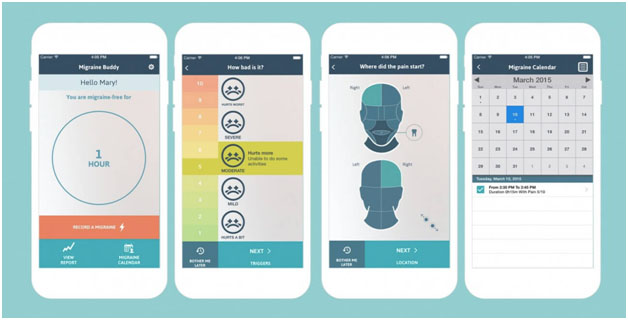
\includegraphics[scale=.3]{./490/migrainebuddy.jpg}
	\caption{Migraine Buddy is condition specific.}
\end{figure}

\section{Team Definition}
Throughout this semester, we utilized digital tools that have version control and allow remote collaboration. This was possible through the use of Github, Hackpad, Google Documents, and Google Hangouts.

\begin{itemize}
\item Github is a version control software that stores iterations of code and allocates space in a centralized location.  This prevents us from working on delayed version of code with our system of emailing source code from one group member to another.

\item Hackpad is a collaborative platform that is analogous to a notepad or a sticky note. This tool was used for regularly accessed data like tutorials and instructions on how to get on the server.  Also, we used this to brainstorm and flesh out ideas before it was finalized in our reports in Google Docs.

\item Google Docs is a collaborative word processor that allows some version control and live updates of shared users. We used this tool for writing and editing reports together and storing official requirements and specifications.

\item Google hangouts is a video call system that allows up to 10 users to be in a call at once per room. This was used as a supplement to our normal weekly meetings on Tuesday and Thursday. We used this time on the google hangout call to troubleshoot github issues, coordinate information retrieval from page to page, and did some rubber duck debugging (talked through difficult problems out loud to get to a solution.)
\end{itemize}

When it came to dividing up the tasks, we analyzed the requirements and specifications of the project and brainstormed all the possible pages that would be needed for full functionality. We then split up the pages based on how the pages interacted with user data. Pages that had similar structure were grouped together to create consistent code. 

\begin{table}[]
\centering
\caption{Initial distribution of work.}
\label{my-label}
\begin{tabular}{|l|l|}
\hline

Lauren Whitesell                                                                                                     & Curtis Sunley                                                                                                           \\ \hline
\begin{tabular}[c]{@{}l@{}}resetpass\\ allergies page\\ medication page\\ unit tests\\ table management\end{tabular} & \begin{tabular}[c]{@{}l@{}}forgotpass\\ add new person\\ add existing person\\ unit tests\end{tabular}                  \\ \hline

Sophia Thach                                                                                                         & Kendall Pitts                                                                                                           \\ \hline
\begin{tabular}[c]{@{}l@{}}index/login\\ menus\\ password (hash/salt)\\ unit tests\end{tabular}                      & \begin{tabular}[c]{@{}l@{}}editaccount\\ editperson\\ myportal \\ register\\ unit tests\\ table management\end{tabular} \\ \hline
\end{tabular}
\end{table}

Each of us were assigned individual tasks, but as the semester progressed, we began to add more features, like the journal and calendar, that required more collaboration and communication between each other.  We had to make decisions that could potentially affect the functionality of another page for which we did not have ownership. We had the opportunity to either work with the our team member’s code or alter their code to fit our own code, depending on which opportunity was the most beneficial to the project.

\section{Requirements}
From a testing to a production environment, MedaWiGi did not have many dependencies or components that were necessary for the project to function. All server-side logic was written in PHP, and JavaScript/HTML 5/CSS 3 was used for the client side markup and scripts. For the calendar functionality, JQuery was necessary for handling Ajax requests and populating the calendar events with entries for the user’s journal. For local testing, the XAMPP Apache distribution was an invaluable tool. The necessary components of the distribution were PHP 5.6.14, a MySQL database, and phpMyAdmin. phpMyAdmin specifically was very helpful in visualizing our SQL tables and making sure records were updating accordingly when testing locally. For our production environment, a LAMP server (Linux, Apache, MySQL, PHP) was used to house our application.

\section{Design}
In the initial stages of MedaWiGi, we adopted a MVC (Model-View-Controller) design pattern and planned to separate our server and client-side logic, and our database. In reality, the architecture of our project blended the View and Controller aspects of MVC, with HTML and PHP server code sitting in the same files, while the Model was our MySQL database. On the LAMP server, there are some PHP scripts that are hidden from view, namely those that deal with email functions (both receiving emails from users and sending them), and our script that connects to the database. While functional, this is not an optimal, nor safe design, and neither is it what we originally intended. Having a much more modular design, where we could call on different scripts inside our HTML pages instead of having to write similar functions on each page was our original goal. 

The View-Controller components represent the majority of MedaWiGi’s PHP files, with every forward-facing web page adopting this design. Each page has their necessary scripts wrapped inside PHP tags right below, or above the HTML. In some cases, the HTML and PHP are blended, in order to dynamically generate markup elements such as tables or labels through the “echo” functions. For example, the “Forgot Password” page will echo a specific secret question and accompanying form for the secret answer, based on what email address is entered into a prior form on the page.

Our Model was a MySQL database that holds the entirety of our user records in multiple tables. Each major feature of MedaWiGi has its own table to store data, including registered users (accounts) and persons (either registered, or non-registered persons using MedaWiGi to store information). To complement our unique feature of adding linking registered users or adding persons to another user's account, a table specifically designed to link people to a registered account was needed, and therefore implemented. 

\begin{figure}[!htb] 
	\centering
	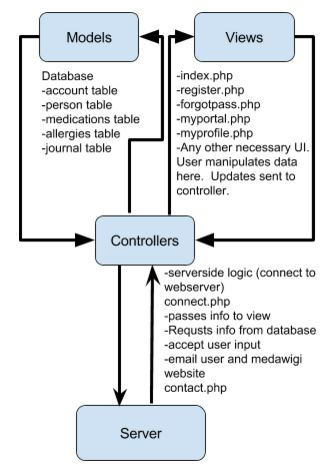
\includegraphics[scale=1]{./490/MVC2.jpg}
	\caption{Draft Model featuring the Model View Controller pattern.}
\end{figure} 

\section{Data Management}
The data was organized into ten tables with the potential to increase this number if additional features were added to the project. The accounts table contains account information, which is the data associated with registered users such as login information and security features like secret questions and answers. The persons table contains profile information. This is the data associated with the profiles under an account including name, date of birth, and avatar. The relationship between the accounts table and the persons table is many-to-many due to the fact that registered users’ profiles can be linked to other accounts, and this is regulated by a mappings table. The mappings table is organized by the accountID, automatically generated by the accounts table. Each entry includes all personIDs, automatically generated by the persons table, that are associated with a given account.

Flags are placed on the linked profiles to differentiate them from the original profiles in an account. The flags are necessary to determine which personIDs should be deleted when a profile is removed from an account. For instance, if a linked profile was removed, the personID on the account which created it should remain untouched, but if an original profile was removed, all personIDs associated with that profile should be deleted from the table. The flags could also be used to set up permissions later. In addition to being used on the mappings table, the accountIDs and personIDs are used as keys for the other tables. The events table, which is used by the calendar and the journal, is tied to the accountID since it is only necessary to have one calendar for each account. All the other tables: medications, contacts, immunizations, conditions, insurance, and allergies, use the personID.

All values in the accounts table are required from the user when they initially register their account, but this action actually populates three tables. In addition to creating an entry in the accounts table, it also automatically generates a new profile in the persons table, and the accountID and personID are placed into the mappings table. The add profile option only updates two tables, the persons table and the mappings table. In contrast, the other tables are more flexible since the information they contain is accumulated gradually over a lifespan rather than at account or profile creation. All of the inputs for all of the tables are accepted from the user as strings, this includes the avatar on the persons table since the decision was made to only store the path to the image in the table.

\section{Implementation}
For the implementation, the project was divided into tasks and these tasks were given a priority level. The first-order priorities were given to infrastructure projects which dealt with account information such as login, logout, registration, and forgot password. Any features that handled creating or deleting a profile were also considered first-order priorities. The second-order priorities were assigned to features that increased the functionality of the project. These included the menu, calendar, and other features that managed profile information including medications, allergies, immunizations, and conditions. Additional features, regulated to future work, were given the lowest priority level.

Computing requirements for the project were minimal since HTML 5 is supported on all modern browsers. It is necessary for the user to have a web browser with JavaScript enabled. 

The software was tested manually. As the pages were created, each team member would do independent unit testing on their pages to make sure they operated as intended using their local MySQL database to handle table data. Integration testing was also handled locally due to the use of collaboration tools such as GitHub. After the infrastructure elements were completed, the team moved the entire project to the server and started working directly with the operating website. As the second-order priorities were completed, these also underwent extensive testing. Each team member was required to create an account and populate a profile in order to run functional tests to confirm that all the pages were working correctly.

Current software techniques were used in the design and development of the website. Most of the techniques dealt with security features. SQL injection attacks are a common problem with databases, so effort was taken to implement preventive measures, including SQL commands to escape special characters in a string. Also the Model View Controller pattern was used to separate the responsibilities of different components of the application, so the PHP code was separated into a different file than the HTML code on pages that handled private account information such as username and password. Code reuse is incorporated into the project via the include statement. The connect file in particular is included on every page that needs to connect to the server.

Both procedural and object-oriented techniques were used in the implementation of the project. Although PHP supports both procedural and object-oriented techniques, it was used primarily for procedural programming. In this capacity, it was used to break down the programming tasks into a collection of data structures and methods to assist with the extensive data management required by the project. Most of the functions that would normally be handled by objects were managed through the database. On the other hand, the open-source calendar that was incorporated into the project implemented object-oriented techniques to encapsulate its functions.

\section{Evaluation}
Since this application is web-based, the best way to test its full potential was to host it on a server with a webaddress: 
\\
\\
\noindent
https://medawigi.no-ip.org
\\

The specifications of the Hardware that the server was on was a Dell OptiPlex 990 (Core i7-2600 CPU 16GB DDR3, 1TB HDD). The machine was running on a Linux operating system, Ubuntu 14.04 with LAMP stack. The LAMP stack stands for Linux, Apache, MySql, and PHP/Python/Perl with phpMyAdmin. The specifications of those components were  Apache 2.4.7, MySQL 14.14 and PHP 5.5.9. This setup was important to have because it directly translated to our local setup of XAMPP stack which is similar to the LAMP software bundle, but is a cross-platform package(can be used on Linux, Windows, Mac). As we pulled our code onto the server and added the tables in phpMyAdmin, we tested to see if data was streaming and storing in the appropriate locations and compared the behavior of the website on the server to the website on our localhost.  If it was not the case, we debugged appropriately on the server.

The server was connected to the UNCG’s network ISP (152.13.X.X) and is publicly accessible. Since our website was hosted by the server, when a visitor visited our website, MedaWiGi, the webpage went from the user’s ISP to a UNCG router and it sent the request to the server. This component of setup was important in the implementation of our email services like the contact us option for user feedback and the reset password option for users who forgot their password. This capability could not be tested on our localhost, so the results could not be compared. Instead, they consisted of emailing members of the team to ensure that the mail functions worked within our program.

\section{Analysis}
In our system, we utilized encryption to ensure that the data was secure from other users and attackers. Data was retrieved from the user, processed through the encryption and stored in the database. As the user needs the information, the database entry was decrypted and displayed as plain text. Therefore, over the course of the project we analyzed and compared multiple encryption algorithms to integrate into our product. Encryption speed, level of security, and ease of implementation are a few of the characteristics examined for each algorithm.

Two example encryption algorithms that we considered include RC4 and AES (advanced encryption standard). RC4 is a symmetric stream cipher that processes plaintext in small blocks, usually one bit at a time, and produces a pseudorandom stream of bits. AES is a symmetric block cipher that encrypts large blocks of plaintext at a time, as opposed to the bit-sized blocks that RC4 utilizes. The symmetric cryptography that both algorithms employ involve using the same key for both encryption and decryption. This method is much faster than asymmetric cryptography, where the key used for encryption is different than the key used for decryption. RC4 and AES differ in many ways, both possessing advantages and disadvantages. The stream cipher, RC4, has a simple implementation and runs at a faster rate than AES. Unfortunately, it has a major flaw in security. RC4 possesses large classes of weak keys, causing the cipher to behave in undesirable ways. It allows attackers to break the encryption much easier than with other algorithms, like AES. While AES is much more secure, it is more complex and runs slower. Unlike RC4, it includes three block ciphers: AES-128, AES-192, and AES-256. The different AES ciphers represents the three different key sizes that can be used on the 128-bit sized plaintext \cite{rc4} \cite{aes}.

Further analysis shown in ``Analysis and Comparison of Symmetric Key Cryptographic Algorithms Based on Various File Features,” presents a more detailed comparison of encryption algorithms. Data type, data size, data density, and key size are used to analyze what effects encryption speed. When checking whether the encryption rate has any dependency on either of the four conditions tested, all other variables were kept constant to avoid contamination from an unknown variable. Experimentation showed that changing either the data type or the data density of a file does not have any effect on the rate of encryption. Altering the key size only affects the encryption time of block ciphers, and just by a small amount. As the size of the key increases, the time it takes to encrypt increases. Data size is the only variable that has a major effect on the rate of encryption. The larger the file size, the longer it takes to encrypt the file. The research included in the paper also showed how RC4 is a faster encryption algorithm compared to AES \cite{encryption}. However despite this advantage, MySQL provides AES encryption and decryption functions so it is much easier to implement with our code.

\section{Discussion}
MedaWiGi has a bright future ahead of it, with many options for future development and design left to be explored. First and foremost, either having the website be more mobile device responsive, or even having a linked mobile application is all but necessary. Having a web application is an excellent first start, but MedaWiGi at its essence is an application designed to be accessible at any time, in whatever fashion is convenient for its users. In the same vein as having mobile integration, a further feature we wish to explore is the integration of an address book or contacts stored on mobile devices into the application, so users can more easily import persons and link them to their account. Visual improvements include a family tree diagram that displays relationships between a registered user and their linked persons, as well as a wider selection of avatars and the ability to upload personal photos for profile pictures. Finally, the ability to upload medical documents via Dropbox would serve as an alternative to entering in medical information manually, and would create a more fluid experience for our users.

\section{Conclusion}
MedaWiGi was a challenging project for the team, in the sense that it was significantly more complex than projects we had completed for other courses. Its complexity stemmed from the introduction of web design and database management into the project statement, as most of the team lacked experience in these areas. However the project also gave us the opportunity to display skills in software development and programming languages that we had acquired throughout our tenure at UNCG. Although the project had a large scope, the most important functionalities were implemented successfully and infrastructure was established in such a way as to allow the project to grow in the future. Overall the project proved successful as both a product and a demonstration of our abilities.

\section*{Acknowledgement}
The authors would like to thank our professor Dr. Jeng Ding and a select group of individuals without whom this would not have been possible: Tim DeLisle, Jenn Goodman, Nick Ayala, Cory Sabol, and the entire Team Bill.


\clearpage
\onecolumn
\begin{thebibliography}{10}
\raggedright
\small
\bibitem{guevara}
K. Guevara. (2015, Apr. 13). Step-by-Step PHP Tutorials for Beginners [Online]. Available: http://www.codeproject.com

\bibitem{heijnen}
A. Heijnen. (2013). [Online]. Available: https://github.com/zabuto/calendar

\bibitem{encryption}
R. Masram et al., ``Analysis and Comparison of Symmetric Key Cryptographic Algorithms Based on Various File Features," IJNSA, Vol.6, No.4, July 2014.

\bibitem{freehealthtrack}
[Online]. Available: http://www.freehealthtrack.com

\bibitem{ibluebutton}
[Online]. Available: http://www.ibluebutton.com

\bibitem{jsfiddle}
[Online]. Available: http://jsfiddle.net/n2gkm4d9/

\bibitem{migrainebudy}
[Online]. Available: http://www.migrainebuddy.com

\bibitem{mymedical}
[Online]. Available: http://mymedicalapp.com

\bibitem{stackoverflow}
[Online]. Available: http://stackoverflow.com

\bibitem{php}
[Online]. Available: https://php.net/manual/

\bibitem{rc4}
[Online]. Available: http://cryptography.wikia.com/wiki/RC4

\bibitem{aes}
[Online]. Available: http://cryptography.wikia.com/wiki/Advanced\_Encryption\_Standard

\end{thebibliography}
\end{document}


